\section{Android Applikation}
\label{sec:android}

Als Hauptsystem in diesem Projekt wurde eine Applikation für die Android
	Plattform erstellt. Diese Applikation dient der mobilen Überwachung
	von Lieferungen bzw. den Gegenständen einer Lieferung.

Android \footnote{http://www.android.com/} ist ein Betriebssystem sowie auch eine Software Plattform für mobile Geräte.
Es werden Smartphones, Netbooks, Mobiltelefone und Tablets unterstützt. Entwickelt wurde das Betriebssystem von der
\emph{Open Handset Alliance} \footnote{http://www.openhandsetalliance.com/}, einem Konsortium von 80 Firmen zur Schaffung offenen Standards 
für mobile Geräte, die von \emph{Google} im Jahr 2007 gegründet wurde (vlg. \cite{OHA07}). 

Wir entschieden uns für Android, da es die gewünschten Anforderungen an unsere mobile Applikation am besten erfüllt. Die Vorteile bzw. Nachteile 
von Android sind nachfolgend aufgelistet.

\subsubsection*{Vorteile}

\begin{itemize}
 \item Android ist \emph{Open Source} und wird ständig aktualisiert.
 \item Als Programmiersprache wird \emph{Java} eingesetzt.
 \item \emph{CouchDB} ist für Android vorhanden.
 \item Große Community und gut dokumentierte API vorhanden.
 \item \emph{Android SDK} ist als Plugin für \emph{Eclipse} \footnote{http://www.eclipse.org/} verfügbar.
 \item Plattformunabhängige Entwicklung möglich.
 \item Android Smartphones werden von verschiedensten Herstellern angeboten.
 \item Einfaches Deployment der Anwendung mittels \emph{adb} oder \emph{App-Installer}
\end{itemize}

\subsubsection*{Nachteile}

\begin{itemize}
 \item Jeder Fahrer benötigt ein eigenes Android Smartphone.
 \item Durch fehlerhafte Bedienung des Benutzers kann die Funktionsweise der mobilen Applikation beeinträchtigt werden.
\end{itemize} 
	
\subsection{Benutzung}

Nach dem sich der Fahrer mit seinem Benutzernamen, seinem Passwort und der ausgewählten Transporteinheit eingeloggt hat, gelangt er auf den \emph{Home} Screen.

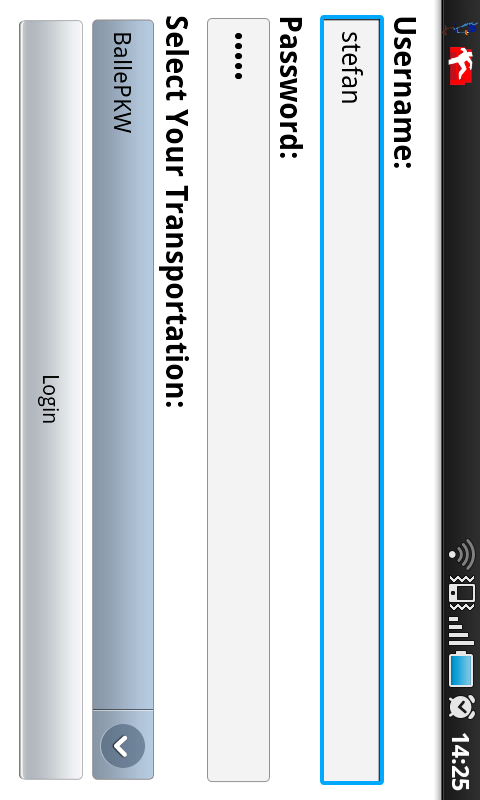
\includegraphics{../files/android_app_login.png}

Die Benutzeroberfläche des \emph{Home} Screens ist einfach und intuitiv gestaltet. Der Fahrer hat dann die Möglichkeit 
Barcodes zu scannen sowie die Lieferdetails zu den aktuell geladenen Paketen anzusehen.

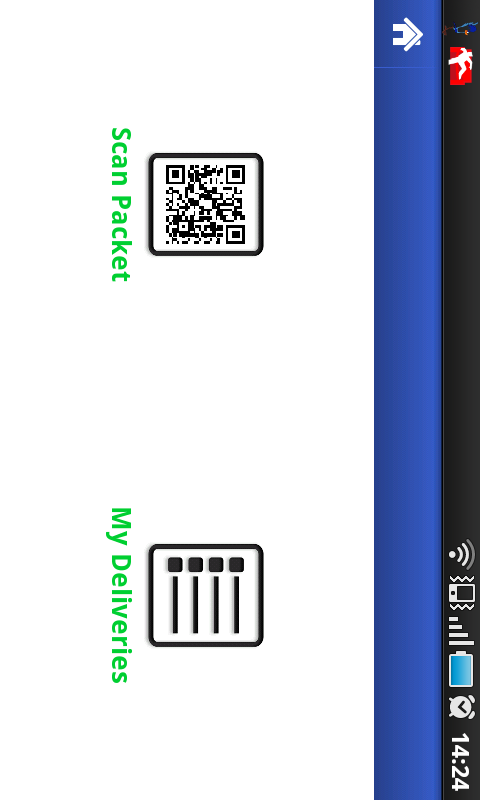
\includegraphics{../files/android_app_home.png}

Nachdem der Barcode eines Pakets gescannt wurde, kann abhängig vom Status des Paketes (aufgeladen - nicht aufgeladen), das Paket
geladen, entladen oder abgeliefert werden. Wenn ein Paket abgeliefert wird, kann der Kunde die Lieferung mit seiner Unterschrift bestätigen.

Mit einem Klick auf den Menüpunkt \emph{My Deliveries} sieht der Fahrer die Adressinformationen des Senders bzw. Empfängers für jede Lieferung.
Weiters können alle Pakete und deren Status einer ausgewählten Lieferung angezeigt werden. 

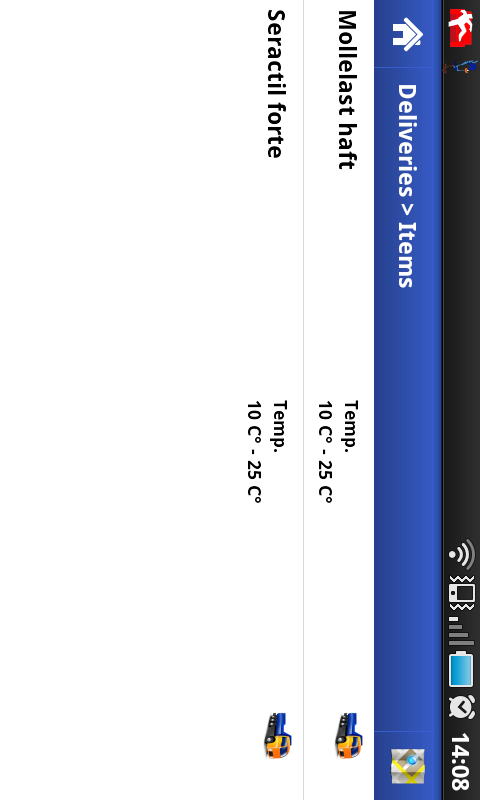
\includegraphics{../files/android_app_deliveries.png}

Außerdem kann die Karte mit der eingezeichnenten Route und der aktuellen Positionen des Fahrers angezeigt werden.

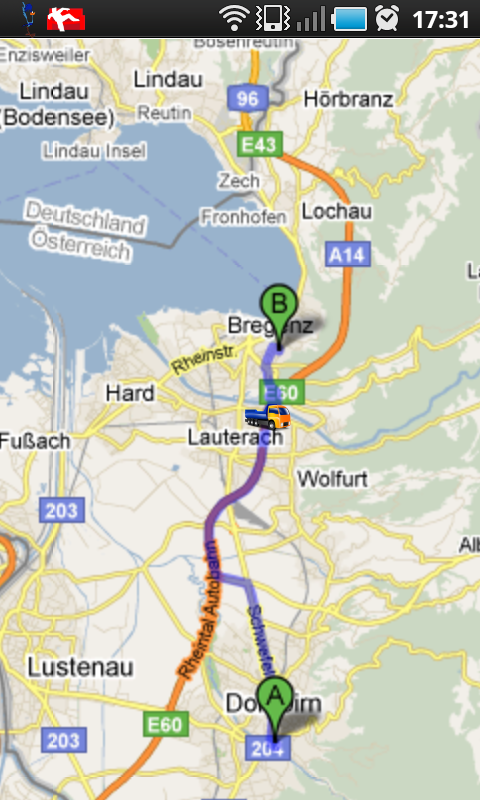
\includegraphics{../files/android_app_map.png}

\subsection{Implementierung}

Bei der Implementierung der Benutzeroberfläche wurden bekannte \emph{UI-Patterns} verwendet. Auf dem \emph{Home} Screen der Applikation
wurde das \emph{Dashboard} Pattern verwendet um die Navigation in der Applikation klar und einfach zu gestalten. Des Weitern enthält jeder
Screen eine \emph{Action Bar} im oberen Teil, die dem Benutzer anzeigt in welchem Kontext der Applikation er sich gerade befindet (\emph{breadcrumbs navigation}).
Mit einem Klick auf das \emph{Home} Symbol in der \emph{Action Bar} hat der Benutzer jederzeit die Möglichkeit wieder auf den \emph{Home} Screen zu gelangen.

Die Dienste zur Überwachung der Temperatur und der GPS-Position sowie zum replizieren der Daten mit der serverseitigen Datenbank sind als \emph{Android Services},
die im Hintergrund laufen, implementiert. Somit wird gewährleistet dass diese wichtige Dienste unabhängig von der Applikation, die auch vom Benutzer geschlossen werden kann,
durchgeführt werden. Diese \emph{Android Services} laufen durchgängig im Hintergrund und müssen explizit beendet werden, falls notwendig.

